\section{Modello di processo}
Come modello di riferimento usiamo il modello agile \textbf{ICONIX}, eventualmente adattando caso per caso le fasi principali.
\begin{figure}[h!] 
	\centering
	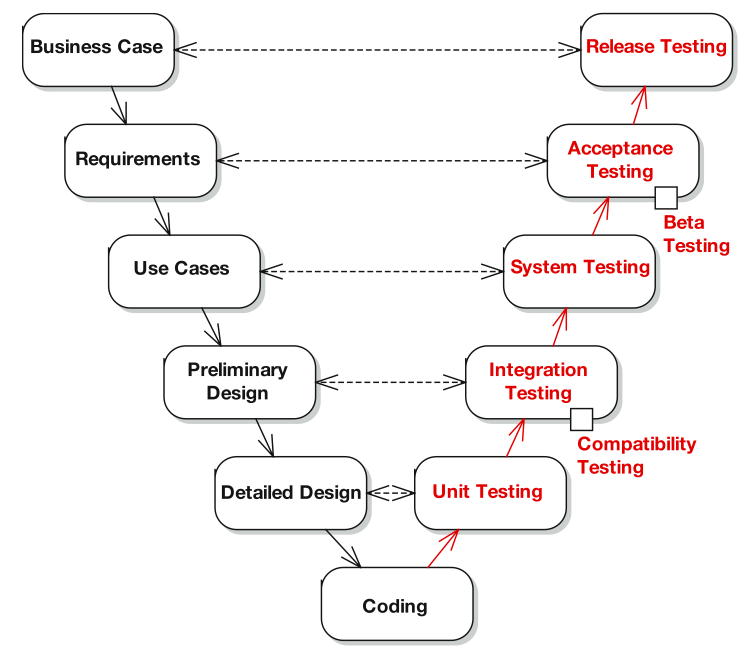
\includegraphics[width=1\textwidth]{gestione_progetto/vmodel.png}
	\caption{Modello a ``V'' che descrive le varie fasi di produzione e di testing}
	\label{fig:vModel} 
\end{figure}
La fase di analisi dei requisiti prevede la produzione dei documenti di domain model, use cases, metriche e mokup.
La fase di progettazione del sistema prevede la produzione dei diagrammi di sequenza e di classe, con descrizioni delle interfacce e degli algoritmi non banali.
La fase di progettazione delle prove prevede la produzione dei robustness diagrams al fine di produrre un documento contenente i test che si vogliono eseguire.